%\documentclass[11pt,a4paper,uplatex,dvipdfmx]{ujarticle} 		% for uplatex
\documentclass[11pt,a4j,dvipdfmx]{jarticle} 					% for platex
%=======================================
% form00_header.tex
%	General header for kakenhiLaTeX,  Moved over from form00_2010_header.tex.
%	2009-09-06 Taku Yamanaka (Osaka Univ.)
%==== General Version History ======================================
% 2006-05-30 Taku Yamanaka (Physics Dept., Osaka Univ.)
% 2006-06-02 V1.0
% 2006-06-14 V1.1 Use automatic calculation for cost tables.
% 2006-06-18 V1.2 Split user's contents and the format.
% 2006-06-20 V1.3 Reorganized user and format files
% 2006-06-25 V1.4 Readjusted all the table column widths with p{...}.
%				With \KLTabR and \KLTabRNum, now the items can be right-justified
%				in the cell defined by p{...}.
% 2006-06-26 V1.5 Use \newlength and \setlength, instead of \newcommand, to define positions.
% 2006-08-19 V1.6 Remade it for 2007 JFY version.
% 2006-09-05 V1.7 Added font declarations suggested by Hoshino@Meisei Univ.
% 2006-09-06 V1.8 Introduced usePDFform flag to switch the form file format.
% 2006-09-09 V1.9 Changed p.7, to allow different heights between years. (Thanks to Ytow.)
% 2006-09-11 V2.0 Added an option to show budget summary.
% 2006-09-13 V2.1 Added an option to show the group.
% 2006-09-14 V2.1.1 Cleaned up Kenkyush Chosho.
% 2006-09-21 V2.2 Generated under a new automatic development system.

% 2007-03-24 V3.0 Switched to a method using "picture" environment.

% 2007-08-14 V3.1 Switched to kakenhi3.sty.
% 2007-09-17 V3.2 Added \KLMaxYearCount
% 2008-03-08 V3.3 Remade it for 2009 JFY version\
% 2008-09-08 V3.4 Added \KLXf ... \KLXh.
% 2011-10-20 V5.0 Use kakenhi5.sty, to utilize array package in tabular environment.
% 2012-08-14 v5.1 Moved preamble and kakenhi5 into the current directory, instead of the parent directory.
% 2012-11-10 v6.0 Switched to kakenhi6.sty.
% 2015-08-26 v6.1 Added KLFirstPageIsLongPage flag.
% 2017-05-27 v7.0 Simplified for the new format.
% 2022-10-27 v7.1 Removed [dvipdfmx] from \usepackage{graphicx}.
%=======================================
% Dummy section and subsection commands.
% With these, some editors (such as TeXShop, etc.) can jump to the (sub)sections.
\newcommand{\dummy}{dummy}% 
\renewcommand{\section}[1]{\renewcommand{\dummy}{#1}}

\usepackage{calc}
\usepackage{geometry}                % See geometry.pdf to learn the layout options. There are lots.
\usepackage{graphicx}
\usepackage{color}
\usepackage{ifthen}
\usepackage{udline}
\usepackage{array}
\usepackage{longtable}
\usepackage{fancyhdr}
 % pieces
%==================================================
% kakenhi7.sty
%==================================================
% v1
% Minimum amount of macros for writing Kakenhi forms.
%
% 2005-10-24 Taku Yamanaka, Physics Dept. Osaka Univ.
%		taku@hep.sci.osaka-u.ac.jp
% 		Macros such as XYBC, etc. were imported from Kakenhi Macro at
% 		http://www.yukawa.kyoto-u.ac.jp/contents/researcher/kakenhi.html .
% 2006-06-04 Taku
%		Added macros to draw boxes if \DrawBox is in the source.
%		This is useful when designing the LaTeX forms.
% 2006-06-14 Taku
%		Added LaTeX macros to add costs 
%		(\KLResetGrandSum, \KLCostItem, \KLSum, \KLGrandSum).
%		Added a macro \Number to supply commas every 3 digits (imported from kkh.mac).
% 2006-06-25 Taku
%		Added \KLTabC, \KLTabR, \KLTabRNum to specify alignments in tables.
%		Please note that \phantom{...} is required for the column, 
%		or otherwise somehow p{...mm} is ignored.
% 2006-08-13 Taku
%		Added \KLItemNumUnitCost . This requires calc.sty.
% 2006-09-06 Taku
%		Added KLGrandTotalValue to add ALL the costs.
%		Also added \KLPrintGrandTotal to print the total on the console.
% 2006-09-09 Taku
%		Added macros to handle "efforts".
% 2006-09-10 Taku
%		Added \KLnewcounter to make series of counters.
%		Modified \KLResetGrandSum and \KLSum to add the sum for 
%		each category and year.
% 2006-09-11 Taku
%		Added \NumC to display LaTeX counter with commas.
% 2006-09-12 Taku
%		Added simple macros to make group table.
% 2006-09-23 Taku
%		Added the 'Fair License' notification.
% 2006-10-22 Taku
%		Initialize KLNumPeople to -1, so that the first header row will not be included in the count.
%====================================================
% v2
% 2007-03-24 Taku
%		Instead of using Kakenhi Macros to position items, 
%		switched to a new method using
%		"picture" environment.  The origin of the coordinate is set to 
%		the lower left corner of the paper.  The positions are given in "points", 
%		as can be read by gv. These methods were suggested by 
%		Tsutomu Sakurai at Saitama Univ..
% 2007-03-30 Taku
%		The sum of each category and year is made using 
%		macros \KLItemCost, etc., instead of \KLSum.  This is a step toward
%		automatically aligning category sums in the same year, in some forms.
% 2007-04-02 Taku
%		Added \KLBudgetMiniTabular, \KLMiniSum, etc. to handle
%		budget tables with multiple category columns.
% 2007-05-04 Taku
%		Added \multicolumnDottedLine .
%==================================================
% v3 
% 2007-08-14 Taku
%		Simplified page handling, by introducing \KLBeginSinglePage,
%		\KLPageRange, etc..
% 2007-09-01 Taku
%		Added a new command, \KLItemNumUnitCostLocation , 
%		and \KLAddCost to clean things up.
% 2007-09-06 Taku
%		Set \KLEven/OddLeft/RightEdge parameters in \KLWaterMark.
%		Without it, if \KLLeftEdge or \KLRightEdge is used inside watermark,
%		it generated a very obscure error message, which was hard to track down.
% 2007-09-09 Taku
%		Removed clearring \thiswatermark in \KLClearWaterMarks.
% 2007-09-12 Taku
%		Added \KLPriorityItemNumUnitCostTwo for Tokusui.
% 2007-09-14 Taku
%		Added \KLItemNumUnitCostTwo for tokutei_koubo.
% 2007-09-17 Taku
%		In \KLAddCost, costs are added only if it is within the defined year range.
% 2008-09-02 Taku
%		  Added \KLMonthPriorityItemNumUnitCostTwo for tokutei_keizoku.
% 2008-09-07 Taku
%		   Use \KLJFY to print year in budget tables.
% 2008-10-21 Taku
%			Added KLItemNumUnitCostInParen for shorei.
% 2009-09-03 Taku
%			Added \dottedLine .
%==================================================
% v4
% 2009-09-06 Taku
%			Added macros for partial typesetting.
% 2009-09-12 Taku
%			Added macros for showing coordinates and edges.
% 2009-09-13 Taku
%			Added macros to show boxes and minipage frames and their corner coordinates.
% 2010-03-04 Taku
%			Moved macros for calculating lengths and positions from form07_header.tex to here.
% 2010-04-11 Taku
%			Added \KLItemCostOne for jisedai, and necessary flags to print budget sums before 
%			the detailed budget table.
%==================================================
% v5
% 2011-10-20 Taku
%			By using array package within tabular environment, the following macros were simplified:
%			\KLTabC, \KLTabR, \KLBudgetMiniTabular, 
%			New Macros:
%			\KLCC, \KLCR
% 2011-10-24 Taku
%			Removed using \KLTabR from most of the budget tables.
% 2011-10-26 Taku
%			Added KLMyBudget.
%			Modified KLYearItemNumUnitCostTwo to just put the JFY if the second item is blank.  (For Kiban S)
% 2012-03-10 Taku
%			Changed the tabcolsep for \KLMyBudget to 0pt.
% 2012-08-14 Taku
%			Moved xxx_forms_pdf and _eps directories to under mother.
% 2012-09-09	Taku
%			Added \KLbibitem(B) and \KLcite(B).
% 2012-09-16	Taku
%			Added \KLOtherApplication, \KLOtherApplicationReasons, and \KLOtherFundReasons
%			for tokusui (and maybe for others in the future).
%==================================================
% v6
% 2012-11-10	Taku
% 			Modified \KLOtherApplicationReasons and \KLOtherFundReasons to make the tables compact.
%			These were in hook3.tex for the 2013 version.
%			Added \KLOtherApplicationDiff for many shumokus.
%			Removed \KLbibitemB and \KLciteB.
%			Changed \KLbibitem to use a dedicated column for numbering.
% 2012-11-11	Taku
%			Added \KLItemSetCostLocationInfo and \KLItemCostInfo.
% 2013-09-19	Taku
%			Added \KLOtherPD and \KLOtherPDShort to enter JSPS PD for other funds.
% 2013-10-02	Taku
%			Changed \KLbibItem, not to use a dedicated column for numbering, 
%			because otherwise the label defined in \label{...} cannot be used in @currentlabel.
% 2014-09-22	Taku
%			Added \KLCL for filling narrow tabular cells in English.  
%			(Suggested by Frank Bennett.)
% 2014-11-08	Taku
%			Added an instruction in \KLCheckPageLimit.
% 2015-08-23	Taku
%			Added NumCk to show numbers divided by 1000 (truncated).
% 2015-08-24	Taku
%			Introduced \KLLongPage and \KLSimpleLongPage to offer floating environment in 
%			single-page-frames.
%=====================================================
% v7
%	Frames are gone!  Simplify kakenhiLaTeX to benefit from 
%	the new style.
% 2017-05-03	Taku
%			Added \KLAnotherFund .
% 2017-05-27	Taku
%			Made \KLBeginSubject and \KLEndSubject to handle new 
%			mother file style.
% 2017-08-17 Taku
%	Added \KLItemCostNoYear and \KLEndBudgetNoYear for kokusai_kyoudou.
% 2017-08-19	Taku
%			Updated \KLBeginSubject and \KLEndSubject to handle 
%			various headers.
% 2017-08-20	Taku
%			\KLBeginSubject calls \KLFirstPageStyle and \KLDefaultPageStyle
%			which should be defined for each shumoku (or JSPS/MEXT).
%			This is to pass the subject name etc. to the header.
% 2017-08-27	Taku
%			Set section number in \KLBeginSubject.
% 2017-08-29	Taku
%			Moved over KLShumokuFirstPageStyle and KLShumokuDefaultPageStyle.
%			Added jsps-abs-p1-header, jps-abs-subject-header, and 
%			jsps-abs-default-header as arguments to \KLShumoku***Header.
% 2017-09-02	Taku
%			Added \KLBeginSubjectWithHeaderCommands for more flexible header style.
% 2017-09-03	Taku
%			Added \vspace*{-4mm} after \includegraphics in \KLBeginSubject*.
% 2017-09-05	Taku
%			Removed now-the-old commands.
% 2020-01-02	Taku
%			Added more numbers to \KLJint for gakuhen_a.
% 2020-01-15	Taku
%			Changed the horizontal position (none --> -3mm) 
%			and the width of the top boxes for headers (\linewidth --> 1.02\linewidth)
%			to reproduce the original boxes.  
%			This became necessary because the margins were set correctly in form02_header.tex.
% 2021-01-29	Taku
%			Set section counter and reset subsection counter only if the section # is given for
%			\KLBeginSubject and \KLBeginSubjectWithHeaderCommands .
% 2022-01-26	Taku
%			Changed the scale for the top boxes from 1.03 to 1.01, 
%			and \hspace from -3mm to -2mm.  (DC)
% 2022-02-23	Taku
%			Introduced \KLBoxOffset and \KLBoxScale for flexibility.
% 2022-03-20	Taku
%			Added '%' after \hspace{ } before incldegraphics.
% 2022-08-03	Taku
%			Use width=\KLBoxWidth, instead of \KLBoxScale*\linewidth which depents on
%			\linewidth.  (I should have noticed it earlier.)
% 2023-03-09	Taku
%			Added \vspace*{\KLBoxVOffset} to \KLBeginSubject.
% 2023-07-10	Taku
%			Added \includegraphics_full_width to place full-width 
%			instruction box images.
%			This is used also for \KLBeginSubject and 
%			\KLBeginSubjectWithHeaderCommands.  
%			\KLBoxOffset and \KLBoxWidth are not needed anymore.
%			Why didn't I think of it (-1in-\oddsidemargin) before??
% 2023-07-18	Taku
%			Old LaTeX cannot handle \hspace{-1in-\oddsidemargin}.
%			Changed to calculate the length by \setlength, and then use the result in \hspace.
%=====================================================

%=====================================================
% Macro to supply commas every 3 digits (up to 9 digits)
%	Imported from kkh.mac for Kakenhi Macro.
%=====================================================
%
\newif\ifNumWithCommas \NumWithCommastrue
\def\NumWithCommas{\NumWithCommastrue}
\def\NumWithoutCommas{\NumWithCommasfalse}
\newcount\Numa
\newcount\Numb
\def\Numempty{}%output blank if "-0" is given
\def\Number#1{\edef\Numpar{#1}\ifx\Numempty\Numpar\else%
\ifNumWithCommas\Numa=#1\relax
\ifnum\Numa>999999\divide\Numa by 1000000
\number\Numa,%
\multiply\Numa by -1000000\advance\Numa by #1\relax
\Numb=\Numa\divide\Numa by 1000
\ifnum\Numa<100 \ifnum\Numa<10 0\fi0\fi\number\Numa,%
\multiply\Numa by -1000\advance\Numa by \Numb
\ifnum\Numa<100 \ifnum\Numa<10 0\fi0\fi\number\Numa%
\else\ifnum\Numa>999\divide\Numa by 1000
\number\Numa,%
\multiply\Numa by -1000\advance\Numa by #1\relax
\ifnum\Numa<100 \ifnum\Numa<10 0\fi0\fi\number\Numa%
\else\number\Numa\fi\fi\else\number#1\fi\fi}

%======================================================
% Macro to display LaTeX counter with commas every 3 digits.
%======================================================
\newcommand{\NumC}[1]{\Number{\value{#1}}}

\newcounter{kyen}
\newcommand{\NumCk}[1]{%
	\setcounter{kyen}{\arabic{#1}/1000}
	\Number{\value{kyen}}
}

%======================================================
% Macros to align (right-justify, center) elements within a tabular cell
% whose width is defined by p{...}.
% 2006-06-25 Taku
% 	These are necessary, because the cell width should be given explicitly
% 	by p{...mm} to match the given table in a tabular environment.  
% 	One could allocate a width with \phantom{...},
% 	but it is a little tricky, since it depends on the font size.
%======================================================

%---------------------------------------------------------------------
% Center text within a tabular cell allocated by p{...}
%\newcommand{\KLTabC}[1]{\multicolumn{1}{c}{#1}}
\newcommand{\KLTabC}[1]{\centering\arraybackslash#1}
% This new method does not require a dummy table row to put them in correct columns.
%
% This should be used in tabular definition, as:
%	\begin{tabular}[t]{>{\KLCC}p{30pt}p{50pt}}
\newcommand{\KLCC}{\centering\arraybackslash}

%---------------------------------------------------------------------
% Right justify text within a tabular cell allocated  by p{...}
%\newcommand{\KLTabR}[1]{\multicolumn{1}{r@{\ }}{#1}}
\newcommand{\KLTabR}[1]{\raggedleft\arraybackslash#1}

% This should be used in tabular definition, as:
%	\begin{tabular}[t]{>{\KLCR}p{30pt}p{50pt}}
\newcommand{\KLCR}{\raggedleft\arraybackslash}%

%---------------------------------------------------------------------
% Right justify number (with comma every 3 digits) 
% within a tabular cell allocated by p{...}
\newcommand{\KLTabRNum}[1]{\KLTabR{\Number{#1}}}

%---------------------------------------------------------------------
% Left justify text within a tabular cell allocated by p{...}
% This should be used in tabular definition, as:
%	\begin{tabular}[t]{>{\KLCL}p{30pt}p{50pt}}
\newcommand{\KLCL}{\raggedright\arraybackslash}%

%=================================================
%  counter tools
%=================================================
\newcounter{KLtmp}

%------------------------------------------------------------------------------
% Makes a set of counters, with prefix #1, followed by 
% suffix ranging from 0 to #2 - 1.
% For example, \KLnewcounter{mine}{3} makes counters
% mine0, mine1, and mine2 .
%-------------------------------------------------------------------------------
\newcommand{\KLnewcounter}[2]{
	\setcounter{KLtmp}{0}
	
	\whiledo{\value{KLtmp} < #2}{
		\newcounter{#1\arabic{KLtmp}}
		\stepcounter{KLtmp}
	}
}

%------------------------------------------------------------------------------
% Dumps the contents of the counters.
%------------------------------------------------------------------------------
\newcommand{\KLdumpcounter}[2]{
	\setcounter{KLtmp}{0}
	
	\whiledo{\value{KLtmp} < #2}{
		#1\arabic{KLtmp} : \arabic{#1\arabic{KLtmp}}\\
		\stepcounter{KLtmp}
	}
}

%=======================================================
% LaTeX macros to add costs.
%	2006-06-14 Taku Yamanaka
%=======================================================
\newcounter{KLCost}				% to calculate cost = #units x unit cost
\newcounter{KLGrandTotalValue}		% for the grand total of all the categories in all years
\setcounter{KLGrandTotalValue}{0}

\newcommand{\KLCostCategory}{KLequipments}
\newcounter{KLYearCount}
\newcounter{KLPrintYear}

% Make counters for annual sums for each category-----------------------
\newcommand{\KLMaxYear}{8}
\KLnewcounter{KLequipments}{\KLMaxYear}
\KLnewcounter{KLexpendables}{\KLMaxYear}
\KLnewcounter{KLdomestic}{\KLMaxYear}
\KLnewcounter{KLforeign}{\KLMaxYear}
\KLnewcounter{KLtravel}{\KLMaxYear}
\KLnewcounter{KLgratitude}{\KLMaxYear}
\KLnewcounter{KLmisc}{\KLMaxYear}
\KLnewcounter{KLAnnualSum}{\KLMaxYear}

%------------------------------------------------
% Add up the given cost to category-year sum, category sum, year-sum, and total.
% 2007-09-01 Taku
% 2007-09-17 Taku: Add costs only if it is within the defined year range.
%------------------------------------------------
\newcommand{\KLAddCost}[1]{%
	\ifthenelse{\value{KLYearCount} > \value{KLMaxYearCount}}{%
		%pass
	}{%
		\addtocounter{\KLCostCategory0}{#1}%
		\addtocounter{\KLCostCategory\arabic{KLYearCount}}{#1}%
		\addtocounter{KLAnnualSum\arabic{KLYearCount}}{#1}%
		\addtocounter{KLAnnualSum0}{#1}%
		\ifthenelse{\equal{\KLCostCategory}{KLdomestic}}{%
			\addtocounter{KLtravel0}{#1}%
			\addtocounter{KLtravel\arabic{KLYearCount}}{#1}%
		}{}%
		\ifthenelse{\equal{\KLCostCategory}{KLforeign}}{%
			\addtocounter{KLtravel0}{#1}%
			\addtocounter{KLtravel\arabic{KLYearCount}}{#1}%
		}{}%
	}%
}


\newcommand{\KLClearWaterMarks}{%
	%--empty watermarks
	\watermark{}
%	\thiswatermark{}
	\rightwatermark{}
	\leftwatermark{}
}

\newcommand{\KLInput}[1]{%	The macros defined inside the file are only valid within the file.
	\begingroup
	\input{#1}
	\endgroup
}

%================================
% For 2017 new style without frames
%================================
\newcommand{\KLShumokuFirstPageStyle}[5]{%
%	Defines the header for the first page.
%	Called from \KLBeginSubject.
%--------------------------------
%	#1: page style name
%	#2: 様式
%	#3: 研究種目名
%	#4: 項目名
%	#5: sectionNo
%--------------------------------
	\ifthenelse{\equal{#1}{jsps-p1-header}}{%
		\JSPSVeryFirstPageStyle{#1}{#2}{#3}{#4}{#5}
	}{%
		\ifthenelse{\equal{#1}{jsps-abs-p1-header}}{%
			\JSPSVeryFirstPageStyle{#1}{#2}{#3 概要}{#4}{#5}
		}{%
            		\ifthenelse{\equal{#1}{jsps-subject-header}}{%
            			\JSPSFirstSubjectPageStyle{#1}{#2}{#3}{#4}{#5}
            		}{%
				\ifthenelse{\equal{#1}{jsps-abs-subject-header}}{%
            				\JSPSFirstSubjectPageStyle{#1}{#2}{#3 概要}{#4}{#5}
				}{%
                    			\thispagestyle{#1}
				}
            		}
		}
	}
}

\newcommand{\KLShumokuDefaultPageStyle}[5]{%
%	Defines the default header.
%	Called from \KLBeginSubject.
%--------------------------------
%	#1: page style name
%	#2: 様式
%	#3: 研究種目名
%	#4: 項目名
%	#5: sectionNo
%--------------------------------
	\ifthenelse{\equal{#1}{jsps-default-header}}{%
		\JSPSDefaultPageStyle{#1}{#2}{#3}{#4}{#5}
	}{%
		\ifthenelse{\equal{#1}{jsps-abs-default-header}}{%
			\JSPSDefaultPageStyle{#1}{#2}{#3 概要}{#4}{#5}
		}{%
            		\pagestyle{#1}
		}
	}
}

\newcommand{\KLSubjectName}{}
\newcommand{\KLSubjectMaxPages}{}
\newcommand{\KLSubjectEndPage}{}
\newcounter{KLSubjectEndPage}
\setcounter{KLSubjectEndPage}{0}

\newcommand{\KLSubjectCheckNPages}{%
%	\arabic{page}, \arabic{KLSubjectEndPage}\\
	\ifthenelse{\value{page}>\value{KLSubjectEndPage}}{
		{\LARGE「\KLSubjectName」は \KLSubjectMaxPages\ ページ以内で書いてください。}
		\clearpage
	}{%
	}
}

\newcommand{\KLSubjectAdvancePages}{%
	\renewcommand{\KLSubjectEndPage}{\value{KLSubjectEndPage}}
	\ifthenelse{\value{page}<\KLSubjectEndPage}{%
		\phantom{x}\clearpage
	}{}
	% Advance page if necessary
	\ifthenelse{\value{page}<\KLSubjectEndPage}{%
		\phantom{x}\clearpage
	}{}
	% Advance page if necessary
	\ifthenelse{\value{page}<\KLSubjectEndPage}{%
		\phantom{x}\clearpage
	}{}
	% Advance page if necessary
	\ifthenelse{\value{page}<\KLSubjectEndPage}{%
		\phantom{x}\clearpage
	}{}
	% Advance page if necessary
	\ifthenelse{\value{page}<\KLSubjectEndPage}{%
		\phantom{x}\clearpage
	}{}
}	

\newcommand{\KLJInt}[1]{%
% Returns full-width numerical character.
	\ifthenelse{\equal{#1}{1}}{1}{%
	\ifthenelse{\equal{#1}{2}}{2}{%
	\ifthenelse{\equal{#1}{3}}{3}{%
	\ifthenelse{\equal{#1}{4}}{4}{%
	\ifthenelse{\equal{#1}{5}}{5}{%
	\ifthenelse{\equal{#1}{6}}{6}{%
	\ifthenelse{\equal{#1}{7}}{7}{%
	\ifthenelse{\equal{#1}{8}}{8}{%
	\ifthenelse{\equal{#1}{9}}{9}{%
	\ifthenelse{\equal{#1}{10}}{10}{%
	\ifthenelse{\equal{#1}{11}}{11}{%
	\ifthenelse{\equal{#1}{12}}{12}{%
	\ifthenelse{\equal{#1}{13}}{13}{%
	\ifthenelse{\equal{#1}{14}}{14}{%
	\ifthenelse{\equal{#1}{15}}{15}{%
	\ifthenelse{\equal{#1}{16}}{16}{%
	\ifthenelse{\equal{#1}{17}}{17}{%
	#1}}}}}}}}}}}}}}}}}%
}

\newlength{\KLFWHOffset}

\newcommand{\includegraphicsFullWidth}[1]{%
	\noindent%
%	\hspace{-1in-\oddsidemargin}%	New LaTeX (2020) can handle this, but old ones (2018) cannot.
	\setlength{\KLFWHOffset}{-1in-\oddsidemargin}%
	\hspace{\KLFWHOffset}%		For old LaTeX
	\includegraphics[width=\paperwidth]{#1}%
}

\newcommand{\KLBeginSubject}[8]{%
%----------------------------------------------------
%	#1: subjectNo
%	#2: sectionNo
%	#3: sectionJ
%	#4: maxPages
%	#5: pageLengthStyle ('V' for variable, 'F' for fixed)
%	#6: pageCounter (set page counter to this value if the argument exists.
%	#7: subjectFirstPageHeader (header for the first page)
%	#8: defaultPageHeader
%----------------------------------------------------
	\ifthenelse{\equal{#2}{}}{%
	}{%
	    	\setcounter{section}{#2}
	    	\setcounter{subsection}{0}
	}
	\setcounter{subsubsection}{0}
	\renewcommand{\KLSubjectName}{#3}
	\renewcommand{\KLSubjectMaxPages}{#4}
	
	\ifthenelse{\equal{#6}{}}{%
	}{%
		\setcounter{page}{#6}
	}
	
	\setcounter{KLSubjectEndPage}{\value{page}}
	\addtocounter{KLSubjectEndPage}{#4}
	
	\ifthenelse{\equal{#7}{}}{%
		% pass
	}{%
		\KLShumokuFirstPageStyle{#7}{\様式}{\研究種目header}{#3}{#2}
	}
	
	\ifthenelse{\equal{#8}{}}{%
		% pass
	}{%
		\KLShumokuDefaultPageStyle{#8}{\様式}{\研究種目header}{#3}{#2}
	}
	
	\vspace*{\KLBoxVOffset}%
%	\noindent
%	\hspace{\KLBoxOffset}%
%	\includegraphics[width=\KLBoxScale\linewidth]{subject_headers/\KLYoshiki_#1.pdf}\\
	\includegraphicsFullWidth{subject_headers/\KLYoshiki_#1.pdf}
	\vspace*{-4mm}
}

\newcommand{\KLNullHeader}[5]{}
% Dummy command for No header.
% This was introduced to avoid error caused in statement \ifthenelse{\equal{#8}{}} .

\newcommand{\KLBeginSubjectWithHeaderCommands}[8]{%
%----------------------------------------------------
%	#1: subjectNo
%	#2: sectionNo
%	#3: sectionJ
%	#4: maxPages
%	#5: pageLengthStyle ('V' for variable, 'F' for fixed)
%	#6: pageCounter (set page counter to this value if the argument exists.
%	#7: LaTeX command for subjectFirstPageHeader (header for the first page)
%	#8: LaTeX command for defaultPageHeader
%----------------------------------------------------
	\ifthenelse{\equal{#2}{}}{%
	}{%
		\setcounter{section}{#2}
		\setcounter{subsection}{0}
	}
	\setcounter{subsubsection}{0}
	\renewcommand{\KLSubjectName}{#3}
	\renewcommand{\KLSubjectMaxPages}{#4}
	
	\ifthenelse{\equal{#6}{}}{%
	}{%
		\setcounter{page}{#6}
	}

	\setcounter{KLSubjectEndPage}{\value{page}}
	\addtocounter{KLSubjectEndPage}{#4}
	
	#7{#7}{\様式}{\研究種目header}{#3}{#2}
	#8{#8}{\様式}{\研究種目header}{#3}{#2}
	
	\vspace*{\KLBoxVOffset}%
%	\noindent
%	\hspace{\KLBoxOffset}%
%	\includegraphics[width=\KLBoxWidth]{subject_headers/\KLYoshiki_#1.pdf}\\
	\includegraphicsFullWidth{subject_headers/\KLYoshiki_#1.pdf}
	\vspace*{-4mm}
}

\newcommand{\KLEndSubject}[1]{%
%	#1: pageLengthStyle ('V' for variable, 'F' for fixed)
		\clearpage % This should be done to update page counter for checking.
		\KLSubjectCheckNPages
		\ifthenelse{\equal{#1}{F}}{%
			\KLSubjectAdvancePages
		}{%
		}
}

%==================================================
% Miscellaneous macros
%==================================================

%----------------------------------------------------------------------
% Draw dotted lines across a multiple column table
%----------------------------------------------------------------------
\newcommand{\multicolumnDottedLine}[1]{%
%	\multicolumn{#1}{@{\hspace{-2mm}}c}{\dotfill}\\%
	\multicolumn{#1}{@{}c}{\dotfill}\\%
}

\newcommand{\dottedLine}{%
	\\\noindent
	\dotfill\\
}

%----------------------------------------------------------------------
% Solid line
%----------------------------------------------------------------------
\newlength{\KLLineLength}
\newcommand{\solidLine}[1]{
%----------- keep an empty line between here and \noindent so that it works after normal text and list.

	\noindent
	\hspace*{-10pt}
	\rule[10pt]{\textwidth}{#1}% #1 = 0.5pt, ....
	\vspace*{-10pt}
}

\newcommand{\KLLine}{%
	\solidLine{1pt}
}

%----------------------------------------------------------------------
% publication list (Thanks to Tetsuo Iwakuma [bulletin board #876])
%----------------------------------------------------------------------
\newcounter{KLBibCounter}

\makeatletter	
	\newcommand{\KLbibitem}{%
		\stepcounter{KLBibCounter}%
		\let \@currentlabel \theKLBibCounter
		\arabic{KLBibCounter}. %
	}
\makeatother

\newcommand{\KLcite}[1]{[\ref{#1}]}

%==================================================
%Fair License

%<Copyright Information>

%Usage of the works is permitted provided that this
%instrument is retained with the works, so that any entity
%that uses the works is notified of this instrument.

%DISCLAIMER: THE WORKS ARE WITHOUT WARRANTY.

%[2004, Fair License: rhid.com/fair]
%==================================================
% You may edit/modify this package at your own risk.
% If there are important fixes or changes that you think should be 
% reflected in the standard distribution, please notify:
%	taku@hep.sci.osaka-u.ac.jp  .
%==================================================
 % pieces
% form01_header.tex
% 2017-05-28 Split from form00_header.tex to move \input{kakenhiLaTeX7.sty} to mother_1.tex.
% 2021-01-28 Set margins.
% 2022-02-23 Introduced \KLBoxOffset and \KLBoxScale.
% 2023-02-13 Introduced \KLBoxVOffset.
% ===== Parameters for KL (Kakenhi LaTeX) ========================
%%\geometry{noheadfoot,scale=1}  %scale=1 resets margins to 0
\setlength{\unitlength}{1pt}

\newlength{\KLCella}
\newlength{\KLCellb}
\newlength{\KLCellc}
\newlength{\KLCelld}
\newlength{\KLCelle}
\newlength{\KLCellf}

\newcounter{KLMaxYearCount}	% # of years for the proposal
\newcommand{\KLCLLang}{}	% language-dependent left-justification in tabular

% ===== format and header =========
% 2021-01-28: Set it to match the margins (17.4 mm on sides (why??), 20 mm on top and bottom). 
% 		On Word, it is set to 16.2 mm, but setting it as 17.4 reproduces the original.
% A4: 294 mm x 210 mm.  
% LaTeX's default margin is 1 inch = 25.4 mm.
\setlength{\oddsidemargin}{-22pt}	% (17.4 - 25.4) / 25.4 * 72 pt/inch = -26 pt
\setlength{\evensidemargin}{-22pt}
\setlength{\textwidth}{496pt}		% (210 - 17.4*2) / 25.4 * 72 = 503 pt
\setlength{\topmargin}{-67pt}	% This and \headheight determine the actual top margin
\setlength{\textheight}{254mm}		% (294 - 20*2) = 254 mm

\setlength{\headheight}{48pt}
\setlength{\headsep}{3pt}

\cfoot{}
\renewcommand{\headrulewidth}{0pt}

\newcommand{\KLBoxVOffset}{-10pt}
\newcommand{\KLBoxOffset}{-17mm}
\newcommand{\KLBoxScale}{1.313}
\newcommand{\KLBoxWidth}{210mm}

\pagestyle{empty}
% ==== other applications table =========
\newcommand{\KLTableHeaderFont}{\fontsize{8.2}{11}\selectfont}
\newcommand{\KLTableHeaderSmallFont}{\fontsize{7.5}{10}\selectfont}
\newcommand{\KLTableHeaderSmallerFont}{\fontsize{7}{10}\selectfont}

 % pieces
% hook3: after including packages ===================
 % pieces
%#Name: dcs
% form04_dcpd_headers.tex
% 2017-08-20 Taku form04_jsps_header.tex
% 2017-08-29 Taku
%			Added a check against jsps-abs-p1-header.
% 2017-09-02 Taku
%			Added sectionNo to the commands to make them compatible with 
%			\KLBeginSubjectWithHeaderCommands.
%			Use \KLJInt.
% 2018-09-01 Taku
%			Adjusted the heights of the headers by inserting \vspace{-3pt} and \rule.
% 2021-01-28 Taku
%			Modified form04_jsps_header.tex to form04_dcpd_header.tex for the new style.
% 2021-02-03 Taku
%			If 研究種目名 for \DCPDVeryFirstPageStyle is empty, do not add a space
%			before "申請内容ファイル" on the top right.
% 2022-01-23 Taku
%			Added 申請者登録名 at the bottom.
% 2022-01-26 Taku
%			Changed \headerfont size from 10 to 10.5.
%			Use zenkaku font for page number.  (sigh ...)
%
\newcommand{\headerfont}{\fontsize{10.5}{10.5}\selectfont}
\newcommand{\contHeaderFont}{\fontsize{8}{8}\selectfont}
% ===== Headers =====================================
\newcommand{\DCPDVeryFirstPageStyle}[5]{%
%	Defines the header for the very first page of the form.
%	Called from \KLShumokuFirstPageStyle in form04_***.
%--------------------------------
%	#1: page style name
%	#2: 様式
%	#3: 研究種目名
%	#4: 項目名
%	#5: sectionNo
%--------------------------------
	\fancypagestyle{DCPDVeryFirstPageStyle}{% The name is not taken from #1, because 
		\fancyhf{}
		\ifthenelse{\equal{#3}{}}{%
			\newcommand{\spaceBefore申請内容ファイル}{}
		}{%
			\newcommand{\spaceBefore申請内容ファイル}{\ }
		}
        		\fancyhead[R]{\headerfont(#3\spaceBefore申請内容ファイル 申請内容ファイル)\vspace{-23pt}\\
        			\rule{0pt}{0pt}\\}
%		\cfoot{\vspace{-2pt}--\ \thepage\ --}
		\cfoot{\vspace{-2pt}--\ \KLJInt{\thepage}\ --}
		\lfoot{\vspace{-2pt}\hspace{104mm}\underline{申請者登録名            }}
		\rfoot{\vspace{-2pt}\underline{\研究代表者氏名}}
	}
	\thispagestyle{DCPDVeryFirstPageStyle}
}

\newcommand{\DCPDFirstSubjectPageStyle}[5]{%
%	Defines the header for the first page for the subject.
%	Called from \KLShumokuFirstPageStyle in form04_***.
%--------------------------------
%	#1: page style name
%	#2: 様式
%	#3: 研究種目名
%	#4: 項目名
%	#5: sectionNo
%--------------------------------
	\fancypagestyle{DCPDFirstSubjectPageStyle}{%
		\fancyhf{}
%		\cfoot{\vspace{-2pt}--\ \thepage\ --}
		\cfoot{\vspace{-2pt}--\ \KLJInt{\thepage}\ --}
		\lfoot{\vspace{-2pt}\hspace{104mm}\underline{申請者登録名            }}
		\rfoot{\vspace{-2pt}\underline{\研究代表者氏名}}
	}
	\thispagestyle{DCPDFirstSubjectPageStyle}
}

\newcommand{\DCPDDefaultPageStyle}[5]{%
%	Defines the default header for the subject.
%	Called from \KLShumokuDefaultPageStyle in form04_***.
%--------------------------------
%	#1: page style name
%	#2: 様式
%	#3: 研究種目名
%	#4: 項目名
%	#5: sectionNo
%--------------------------------
	\fancypagestyle{DCPDDefaultPageStyle}{%
		\fancyhf{}
		\fancyhead[L]{\contHeaderFont{(#4の続き)}}
%		\cfoot{\vspace{-2pt}--\ \thepage\ --}
		\cfoot{\vspace{-2pt}--\ \KLJInt{\thepage}\ --}
		\lfoot{\vspace{-2pt}\hspace{104mm}\underline{申請者登録名            }}
		\rfoot{\vspace{-2pt}\underline{\研究代表者氏名}}
        }
        \pagestyle{DCPDDefaultPageStyle}
}

 % pieces
% form04_dc_header.tex

% ===== Global definitions for the Kakenhi form ======================
% 基本情報
\newcommand{\様式}{}
\newcommand{\研究種目}{DC}
\newcommand{\研究種目後半}{}
\newcommand{\研究種別}{}
\newcommand{\研究種目header}{\研究種目\研究種別\研究種目後半}

\newcommand{\KLMainFile}{dc.tex}
\newcommand{\KLYoshiki}{dc_header}

%==========================================================
 % pieces
% ===== Global definitions for the Kakenhi form ======================
% 基本情報
%
%------ 研究課題名  -------------------------------------------
\newcommand{\研究課題名}{ミューオン電子転換探索の感度向上に向けた解析手法の開発}

%----- 研究機関名と研究代表者の氏名-----------------------
\newcommand{\研究機関名}{大阪大学}
\newcommand{\研究代表者氏名}{高見 翔太   }
\newcommand{\me}{\underline{\underline{Shohta~Takami}}} 
%inst_general_images.tex
\newcommand{\JSPSInstructions}{%
	\textcolor{red}{(\texttt{\textbackslash JSPSInstructions}をコメントアウトしてください。)}\\
	\includegraphicsFullWidth{subject_headers/inst_general.pdf}
}

\newcommand{\PapersInstructions}{%
	\textcolor{red}{(\texttt{\textbackslash PapersInstructions}をコメントアウトしてください。)}\\
	\includegraphicsFullWidth{subject_headers/inst_papers.pdf}
}

\newcommand{\SelfReviewInstructions}{%
	\textcolor{red}{(\texttt{\textbackslash SelfReviewInstructions}をコメントアウトしてください。)}\\
	\includegraphicsFullWidth{subject_headers/inst_self_review.pdf}
}

 % pieces
% user07_header
% ===== my favorite packages ====================================
% ここに、自分の使いたいパッケージを宣言して下さい。
\usepackage{ulem}
\usepackage{wrapfig}
\usepackage{amssymb}
%\usepackage{mb}
\usepackage{amsmath}
\usepackage{xcolor}
\usepackage{enumitem}
%\DeclareGraphicsRule{.tif}{png}{.png}{`convert #1 `dirname #1`/`basename #1 .tif`.png}
\usepackage{lineno}

% ===== my personal definitions ==================================
% ここに、自分のよく使う記号などを定義して下さい。
\renewcommand{\refname}{}%リファレンスの頭に「参考文献」っていうタイトルつけない
\newcommand{\klpionn}{K_L \to \pi^0 \nu \overline{\nu}}
\newcommand{\kppipnn}{K^+ \to \pi^+ \nu \overline{\nu}}
%\newcommand{\mysection}[2]{\hspace{-12pt}\colorbox[gray]{0.8}{\normalsize{\textbf{\ctext{#1}#2}}}\\}
\newcommand{\mysection}[2]{\hspace{-12pt}\colorbox{cyan!15}{\normalsize{\textbf{\ctext{#1}#2}}}\\}
\newcommand{\mysubsection}[1]{\vspace{-20pt}\subsection*{\colorbox{cyan!15}{\normalsize{#1}}}\vspace{-0.2cm}}
% ----- 業績リスト用 -------------
\newcommand{\paper}[6]{%
	% paper{title}{authors}{journal}{vol}{pages}{year}
	\item ``#1'', #2, #3 {\bf #4}, #5 (#6).			% お好みに合わせて変えてください。
}

\newcommand{\etal}{\textit{et al.\ }}
\newcommand{\ca}[1]{*#1}	% corresponding author;   \ca{\yukawa}  みたいにして使う
\newcommand{\invitedtalk}{招待講演}

\newcommand{\yukawa}{H.~Yukawa}					% no underline
%\newcommand{\yukawa}{\underline{\underline{H.~Yukawa}}}	% with 2 underlines
\newcommand{\tomonaga}{S.~Tomonaga}

\newcommand{\prl}{Phys.\ Rev.\ Lett.\ }		% よく使う雑誌も定義すると楽

% ===== 欄外メモ ==================
\newcommand{\memo}[1]{\marginpar{#1}}
%\renewcommand{\memo}[1]{}	% 全てのメモを表示させないようにするには、行頭の"%"を消す

%\input{../../sample/simple/contents}	% skip
% hook5 : right before \begin{document} ==============
 % pieces

\begin{document}

% hook7 : right after \begin{document} ==============
 % pieces
%#Split: 01_background  
%#PieceName: p01_background
% p01_background_00.tex
\KLBeginSubjectWithHeaderCommands{01}{2}{研究の概要と位置づけ}{1}{F}{3}{\DCPDVeryFirstPageStyle}{\DCPDDefaultPageStyle}

\section{研究の概要と位置づけ}
%    <<最大 1ページ>>

%s03_abst_background
\vspace{-0.2cm}
\uwave{波線部はコメント修正箇所です}\\
\noindent
\underline{\textbf{研究課題名:\研究課題名}}

%begin 研究目的や背景などの概要 ====================
\vspace{0.1cm}
\mysubsection{概要}
%end 研究目的や背景などの概要 ====================

%begin 本研究の着想に至った経緯など ====================
素粒子物理学における標準模型は、物質の最小構成要素である\textbf{素粒子}における基本的な相互作用を記述する理論である。
標準模型は未だ不完全で、\uwave{物質反物質非対称性やニュートリノ振動など説明できない現象が残っ}\\
\uwave{ているため}、新理論の発見が待ち望まれている。
本研究で探索する\textbf{荷電レプトンフレーバー非保存過程}(以下、charged Lepton Flavor Violation:cLFV)は
標準模型では崩壊分岐比が$10^{-54}$以下と非常に強く抑制されている。
一方、多くの新理論内ではこの過程が$10^{-15}$程度の確率で観測可能と示唆されている。
従って、cLFVの発見は標準模型の寄与がなく、\textbf{新物理の直接的な証拠}となる。
COMET実験ではミューオン電子転換過程($\mu^- + N \rightarrow e^- + N$)と呼ばれるcLFVの一種を探索する。
COMET実験は現状のミューオン電子転換過程に対する \uwave{世界最高感度を二桁ほど更新するものとなる}。
\mysubsection{研究の位置付け}
\noindent \textbf{・当該分野の状況}\\
ミューオン電子転換探索の世界最高感度は、先行実験のSINDRUM-I\hspace{-1.2pt}Iでの$7 \times 10^{-13}$であり、発見には至らなかった$^{\cite{SINDRUM}}$。
この測定では連続的なビームを使用したため、ビーム由来の背景事象が常に存在し、ビー
\begin{wrapfigure}[9]{r}{190pt}{}
	\centering
	 \vspace{-0.5cm}
	 \hspace*{-15pt}
	 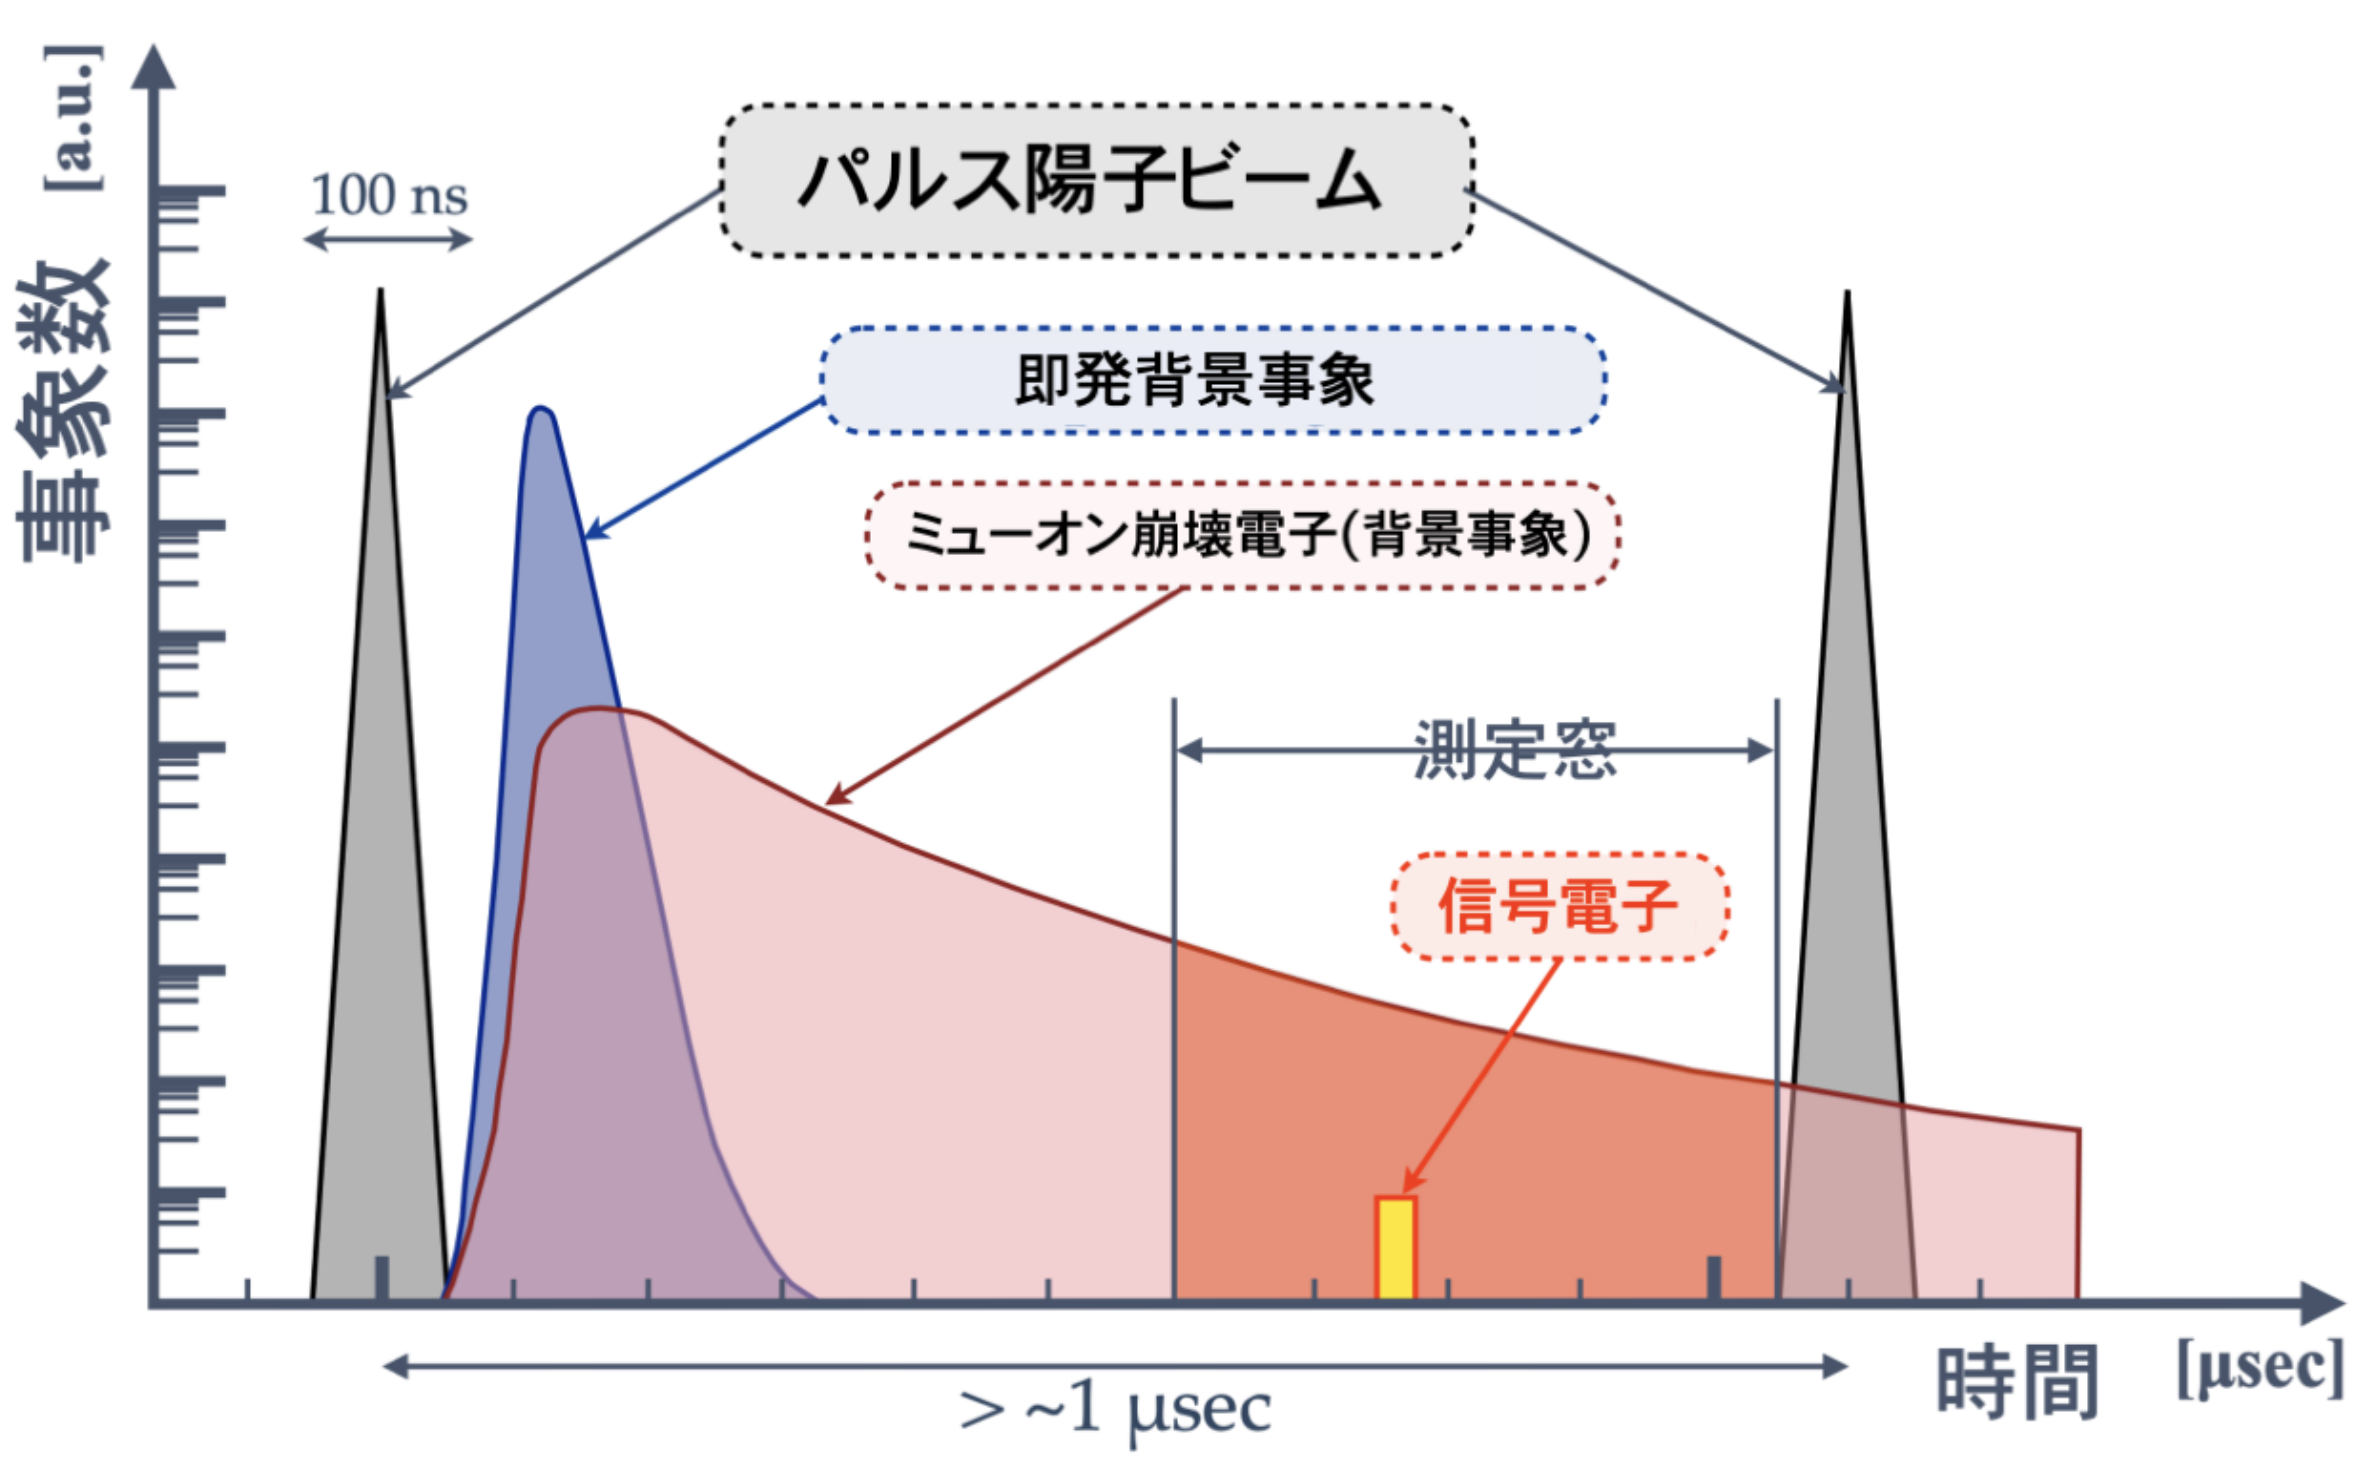
\includegraphics[width=8cm]{figs/beam}
	 \vspace{-1.2cm}
	 \caption{\small{ビームの時間構造}}
	 \label{Fig:beam}
	\end{wrapfigure} 
ム強度に対する探索感度に制限があった。
そこでCOMET実験では、パルス状のビームを使用することと標的にアルミニウムを使用することで背景事象の問題を克服する。
ビームのパルス間隔$1.17\;\rm{\mu s}$に対し、原子中のミューオン寿命が$0.86\;\rm{\mu s}$と長いアルミニウムをミューオン静止標的に採用し、陽子ビームのバンチタイミングから遅れてトリガーをかける。
これにより、ビーム由来のバックグラウンドが大幅に低減する。
同様の実験として米国Fermi研究所にて建設中のMu2e実験$^{\cite{Mu2e}}$があるが、COMET実験が先行して、世界最高感度に到達する計画である。\\
\noindent \textbf{・本研究の着想に至った経緯}\\
COMET実験における背景事象にはビーム由来のもの以外に、原子軌道上におけるミューオンの三体崩壊(Decay In Orbit:DIO)による電子があげられる。
そこで検出された電子の運動量を用いて、DIOによる電子とミューオン電子転換による電子を見分ける。
ミューオンビームのアルミニウム標的への照射は$1\;\rm{T}$のソレノイド磁場内で行う。
そのため、荷電粒子が磁場中で螺旋運動する性質を用いて、運動量を測定することができる。
具体的にはガス飛跡検出器(Cylindrical Drift Chamber:CDC)による電子の飛跡の曲率と磁場の値よりその運動量を測定することができる。
そこで、CDCで検出された背景事象を含むヒットのうち信号電子の飛跡を見つけるアルゴリズムの開発が必要不可欠であり、DIOによる信号と分離するためには\textbf{$\mathbf{200\;\rm{keV/c}}$の運動量分解能}が要求されている。\\
 COMET実験は2026年に全ての装置のインストールが完了し、同年末には低強度ビームでの物理測定を開始し、2028年にはいよいよCOMET Phase-Iが開始する予定である。
従って2026年以降にはCDCの運動量較正や上述の物理解析手法の確立を行うことが優先順位の極めて高い項目である。
そこで、申請者の修士課程における\textbf{磁場分布に関する経験}やトラッキングアルゴリズムに対する理解を活かし、\textbf{世界最高感度でのミューオン電子転換過程探索}を実現する。

%\vspace{1cm}
\small
\begin{thebibliography}{99}
	\bibitem{SINDRUM} SINDRUM-II Collaboration, Eur. Phys. J.C47 337-346 (2006)
	\bibitem{Mu2e}Mu2e Collaboration, Universe, 9, 54. (2023) 
\end{thebibliography}
%\begin{wrapfigure}[9]{r}{190pt}{}
%	\centering
%	 \vspace{-1.1cm}
%	 \hspace*{-15pt}
%	 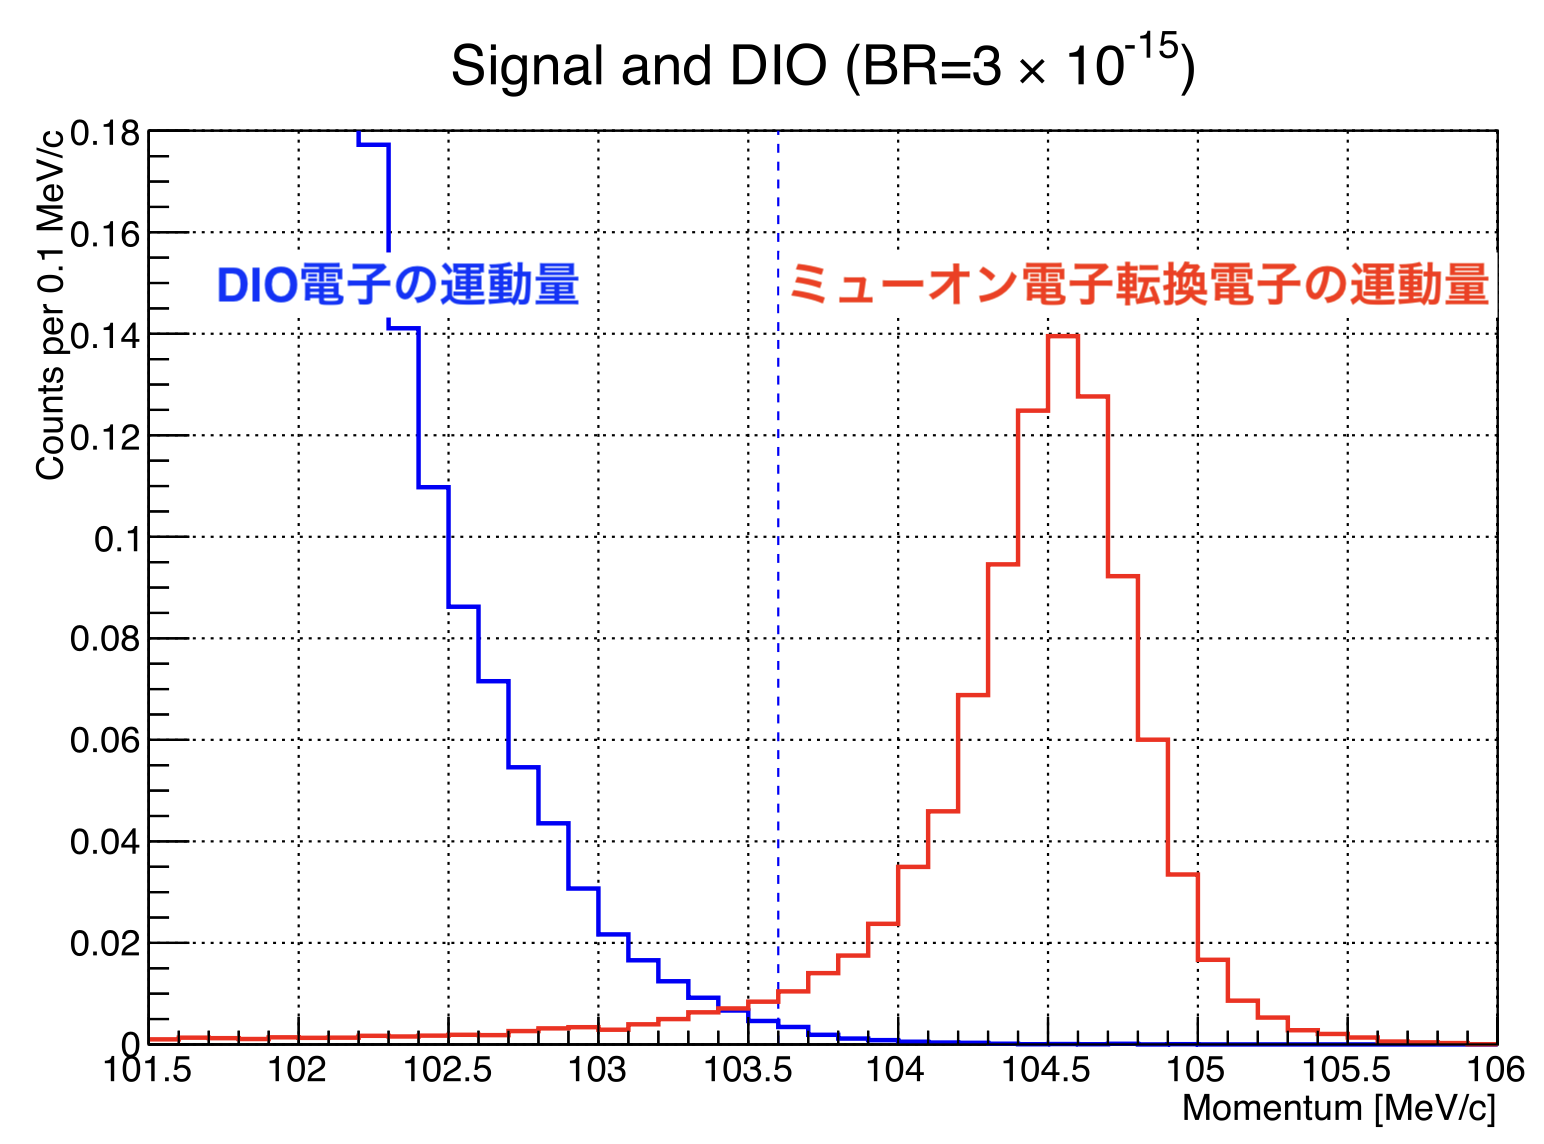
\includegraphics[width=7cm]{figs/momentum.png}
%	 \vspace{-1.2cm}
%	 \caption{\small{運動量分布}}
%	 \label{Fig:beam}
%	\end{wrapfigure} 









%end 本研究の着想に至った経緯など ====================

% p01_background_01.tex
\KLEndSubject{F}


%#Split: 02_purpose_plan  
%#PieceName: p02_purpose_plan
% p02_purpose_plan_00.tex
\KLBeginSubjectWithHeaderCommands{02}{}{【2】研究計画(2)研究目的・内容等}{2}{F}{}{\DCPDFirstSubjectPageStyle}{\DCPDDefaultPageStyle}

\section{【2】研究計画(2)研究目的・内容等}
%    <<最大 2ページ>>
\mysubsection{1.研究目的、研究方法、研究内容}
本研究の目的はミューオン電子転換過程を世界最高感度で探索し、標準模型を破る新物理を実験的に観測することである。
そのため、茨城県の大強度陽子ビーム施設J-PARCで計画している\textbf{COMET実験}で測定および物理解析を主導する。\\
\begin{wrapfigure}[12]{r}{190pt}{}
	\centering
	 \vspace{-1.2cm}
	 \hspace*{-15pt}
	 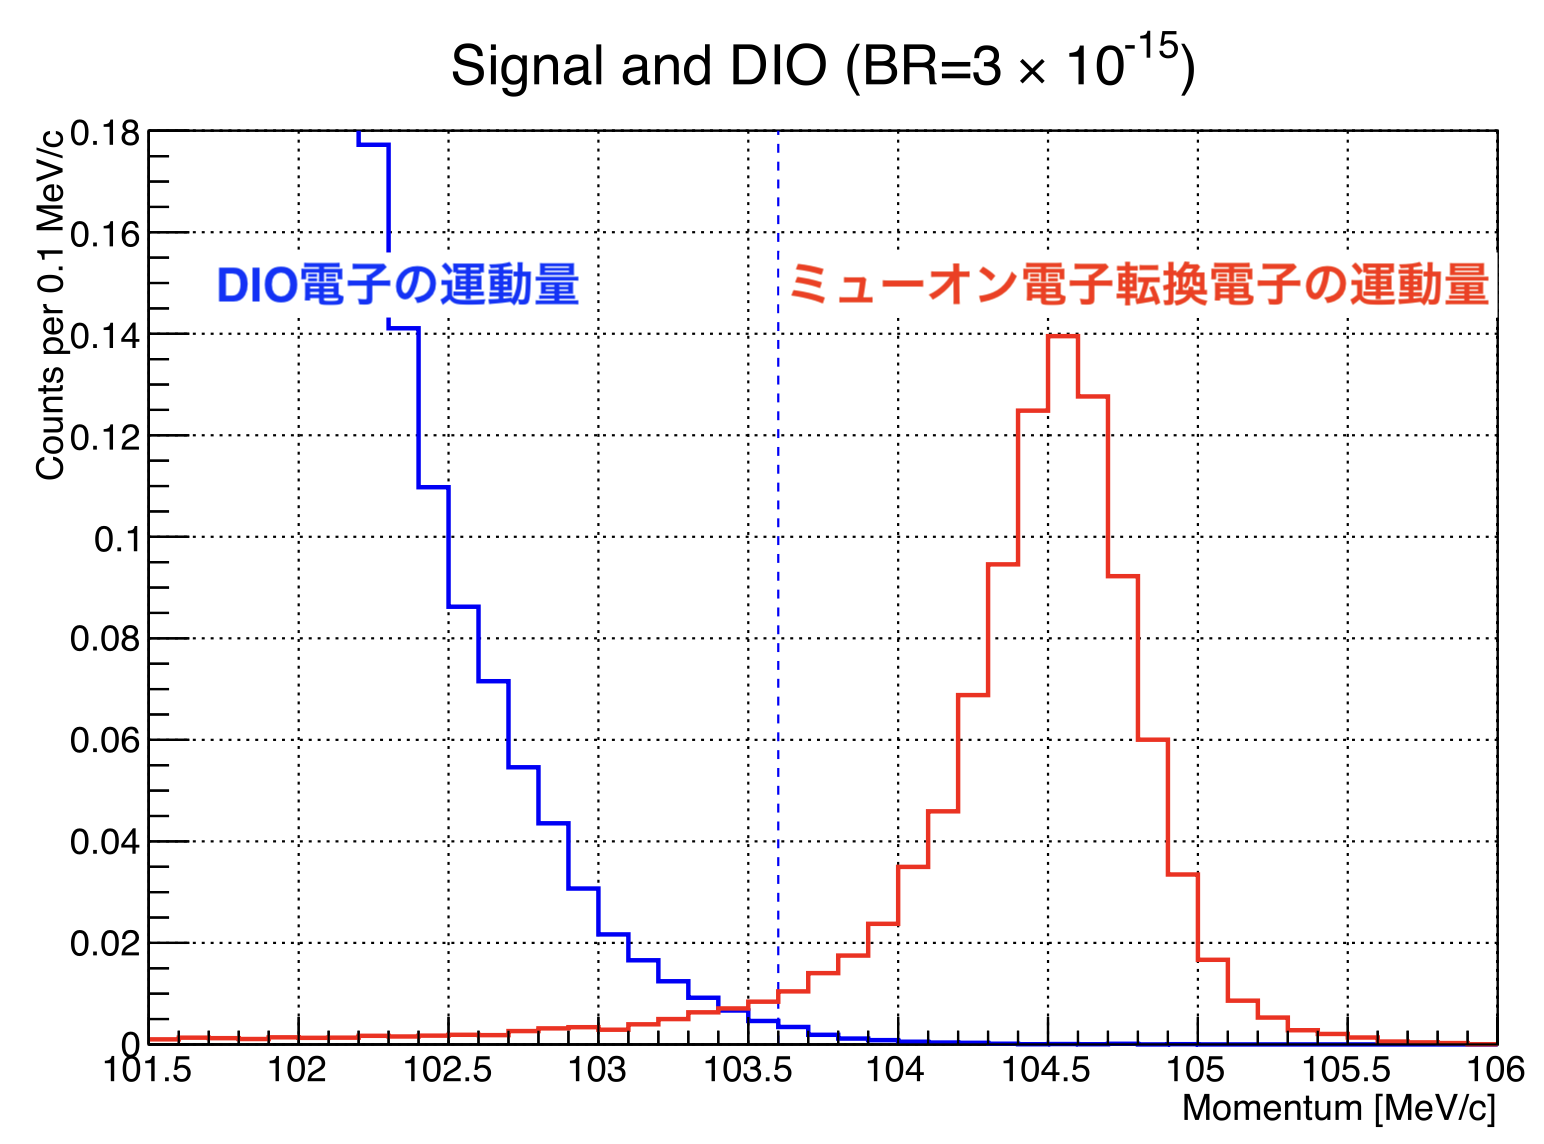
\includegraphics[width=7cm]{figs/momentum.png}
	 \vspace{-1.0cm}
	 \caption{\small{信号電子の運動量分布}}
	 \label{Fig:momentum}
	\end{wrapfigure} 
 アルミニウム原子核に捕獲されたミューオンのミューオン電子転換によって生成される信号電子の運動量はミューオンの質量から原子核の束縛エネルギーと反跳エネルギーを引いた$\mathbf{105\;\rm{MeV/c}}$である。
一方、背景事象である原始軌道上でのミューオンの崩壊(DIO)は三体崩壊であるため、ミューオン電子転換過程よりも小さい運動量になる。
そこで検出器全体をソレノイド磁場内に設置し、粒子の飛跡より求められる\textbf{電子の螺旋運動の曲率}を用いて信号電子の運動量を測定する。
飛跡検出にはガス検出器(CDC)を用い、CDCのデータ取得のトリガーにはシンチレーター検出器CTHを用いる。
図\ref{Fig:momentum}のようにDIO電子と信号電子のスペクトルを分離するには$\mathbf{200\;\rm{keV/c}}$\textbf{の運動量分解能}がCDCには要求されている。\\
%COMET実験は2026年末から低強度ビームでの物理測定、2028年には150日間のビーム運転期間での物理データ測定が予定されている。
%まず、低強度ビームでの物理測定前に、通常のミューオンの崩壊(Mitchel Edge)や$\pi$の$e$への崩壊など標準模型内での電子への崩壊時過程を用いて、検出器の運動量較正を行う。
 信号電子が検出器内で複数周回転するmultiple turn tracksが現在物理解析において問題視されている。その理由は三つあり、第一に、複数周CDCにヒットを残すため、周回ごとにヒットを区別する必要があり、トラッキング精度が悪くなってしまう。
第二に、CDCでのヒットが多い分、失う運動量も大きくなり、DIOとの区別が難しくなる。
第三に、周回が多い分、無関係なノイズを拾いやすい。
結果的に検出器内で一周しかしないsingle turn tracksのアクセプタンスは$11\;\rm{\%}$であるのに対し、multiple turn tracksでは$7.2\;\rm{\%}$になる。
つまり、multiple turn trackを判別できないと、最悪の場合COMET実験で期待できる\textbf{最高感度の2/3}ほどしか達成できない可能性がある。
そこで、multiple turn tracksを判別できる解析法を開発し、\mbox{SINDRUM-I\hspace{-1.2pt}I$^{\cite{SINDRUM}}$}の感度を100倍更新する$\mathbf{3.0 \times 10^{-15}}$での\textbf{ミューオン電子転換過程探索}を実現する。\\
\vspace{-0.5cm}
\mysubsection{2.研究計画}

%\noindent \textbf{【磁場分布の運動量スペクトルへの寄与の評価(採用まで)】}\\
% 信号電子の運動量測定には磁場分布の情報が必要不可欠である。
%申請者は修士課程ではCOMET Phase-Iにおける検出器ソレノイド(Detector Solenoid:DS)の磁場測定に携わっており、
%本番のビームエリアに
%物理ランを行う時のセットアップと同じ本番環境における磁場測定システムの設計には
%運動量分解能$\mathbf{200\;\rm{keV/c}}$を達成するために磁場測定の精度の要求値を決定する必要がある。
%そのために、磁場測定の精度の情報をCOMET実験グループ内で独自に開発されたICEDUST$^{\cite{ICEDUST}}$というGeant4ベースのフレームワークを用いて、シミュレーションを行い、要求されている運動量分解能を満たす磁場測定精度を決定する。
%
\noindent
\textbf{・本番環境での磁場測定(採用まで)}\\
2025年に行われるDSおよびCDCなど検出器のインストールを主導し、実験開始の準備を着実に進める。\\
 信号電子の運動量$p$は磁場$B$と曲率半径$\rho$より、$0.3B\rho$で計算される。
2025年末に行う磁場測定のデータは今後のトラッキングアルゴリズム開発や物理解析に使用するため、\textbf{非常に重要である}。
申請者はCDCに必要な運動量分解能を実現する上で許容される磁場の誤差や要求される精度を、ICEDUST$^{\cite{ICEDUST}}$というフレームワーク(COMET実験グループ内で独自に開発された)を用いて決定している。
この結果に従って要求精度を十分満たす磁場測定システムを開発し、インストール後の2025年末に予定されている本番環境での磁場測定を行う。
ここでは、物理測定時の設定磁場である$1\;\rm{T}$での測定に加え、運動量較正(後述)用の低い磁場(約0.7\;\rm{T}と約0.5\;\rm{T})での測定も加えて行う。
この測定システムの開発には申請者が修士課程1年時に行ったDS納品後の健全性確認のための磁場測定試験で得られた経験が活きると考えている。この経験から得られたフィードバックを活かし、系統的な誤差や揺らぎを最小限に抑え、$200\;\rm{keV/c}$の運動量分解能達成に向けた測定システムを開発する。
\\
\noindent
\textbf{・CDCの運動量較正および宇宙線Run(1年目)}\\
最初に宇宙線を用いた検出器のテスト測定を行う。
この測定では、$2\;\rm{GeV}$程度の信号電子やDIO電子と比べて大きなエネルギーを持つ宇宙線の直線的な飛跡が設計通りの位置分解能で再構成できることを確認する。
これにより、トラッキング性能だけでなく、CTHによるトリガーが機能していること設計通りにデータ取得ができていることも同時に確認できる。
この測定ではハード、ソフト両面での様々な障害が発生することが予想され、各障害の原因特定およびデバッグ作業を行う。\\
 宇宙線でのテスト測定に成功した後は、$\pi$から$e$へのビーム即発背景事象(運動量:$70\;\rm{MeV/c}$)と標準模型内でのミューオンの電子への崩壊(運動量:$52.5\;\rm{MeV/c}$)を用いて、検出器の運動量較正を行う。
信号電子(運動量:$105\;\rm{MeV/c}$)の磁場の強度では飛跡が長くなるため、これらの比較的低運動量電子でも信号電子と同程度の半径の螺旋運動になるように磁場強度を調整する。
その後、同じ条件でトリガーをかけ、CDCでの飛跡検出を行い、運動量較正を行う。
\\
\noindent
\textbf{・低強度ビームでの物理測定およびトラッキングアルゴリズム開発(2年目)}\\
2026年末にCOMET Phase-Iの1/10の強度でビーム供給を行い、物理測定を行う。
現在COMET実験では、検出器内で複数周螺旋運動をするmultiple turn tracksによるアクセプタンスの低下が問題視されている。
実際に電子の螺旋運動を用いて運動量測定を行うMEG実験$^{\cite{MEG}}$でもこの事象は問題視されており、各周回を判別できるようになったことで\textbf{約}$\mathbf{4\;\rm{\textbf{\%}}}$検出効率がアップしたことが報告されている。
しかし、用いるソレノイド磁場の形状が異なるため、COMET実験でも同じ方法を踏襲することはできず、COMET実験独自のアルゴリズムの開発が要求されている。
実際のソレノイド磁場は鉄ヨークに格納されていても完全に一様ではなく、円筒中心軸においてシミュレーション上で磁石中心に対し検出器両端(磁石中心から$1\;\rm{m}$)で\textbf{約}$\mathbf{15\;\rm{\textbf{\%}}}$磁場が低下する。
即ち、$105\;\rm{MeV/c}$の運動量を持った電子では、磁石中心と比較して検出器両端で螺旋運動の半径が\textbf{約}$\mathbf{7\;\rm{\textbf{cm}}}$大きい飛跡を描く。
multiple turn tracksを残すような電子の平均的な円筒軸方向の運動量は約$1\;\rm{MeV/c}$と予想されており、この運動量では螺旋運動一周の間隔は約$2\;{m}$となる。
従って、周回ごとに数cm単位で曲率半径が変化することが予想され、CDCの1セルが$0.16\;\rm{cm}$(%%多分表現正しくないのでSunさんとかに確認します)であることより、
飛跡の曲率半径の違いからmultiple turn tracksの各周回を分離するアルゴリズムを開発する。(%%何%感度が良くなるとか、逆に非一様性のせいでTrack Findingに逆効果があるとかはまだ考えれてないです)
\\
\noindent
\textbf{・Phase-I測定および物理データ解析(3年目)}\\
2028年には予定強度のビームでCOMET Phase-Iの測定が開始するため、2年目までに深めた検出器への理解や低強度ビーム試験時で得たトラブルシューティングの経験を元にこの測定を主導する。\\
 2年目に開発したトラッキングアルゴリズムで実際に得られた物理データの解析を行い、飛跡の再構成の効率やアクセプタンスなどアルゴリズムの性能を評価する。
低強度ビーム試験データを使ったアルゴリズムのブラッシュアップは2028年以降のCOMET Phase-Iでのビーム測定データ解析、ひいてはミューオン電子転換過程発見に繋がる。
(%%コメントもらってたと思うのですが、2026年度のデータを解析し尽くすというところでもう少し相談したいです)

\mysubsection{3.研究の特色、独創的な点}
先行実験の SINDRUM-I\hspace{-1.2pt}I$^{\cite{SINDRUM}}$は連続的なDCビームを使用していたことでビームの強度に対して探索可能な感度に制限があった。
一方、COMETでは世界最高のextinction(時間的純度)のパルスミューオンビームを用い、かつ効率の良い背景事象除去が可能なトリガーシステムを用いることで100倍感度を改善できる。
本研究では、未だ同グループでは着手していない\textbf{ソレノイド磁場の非一様性を利用したトラッキングアルゴリズム開発}を行う。
%また、COMETは本研究におけるPhase-Iからアップグレードを見据えており、さらに100倍感度を更新して、現在の上限値の$10^4$倍の感度で探索を行う予定である。
また、関連実験として同じミューオンcLFVである$\mu \rightarrow e + \gamma$を探索するMEG実験$^{\cite{MEG}}$がある。ガンマを放出するか否かの分岐比は理論依存が大きいため、本
研究の結果と組み合わせることで、より詳細な新物理の検証が可能となる。\\
\mysubsection{4.申請者が担当する部分}
aaaa
\mysubsection{5.異なる研究機関での研究従事}
\small
\begin{thebibliography}{99}
	\bibitem{SINDRUM} SINDRUM-II Collaboration, Eur. Phys. J.C47 337-346 (2006)
	\bibitem{ICEDUST}
  R. Derveni, 
  \emph{Comparative analyses of sub-GeV physics in simulations and data for the COMET experiment},  
  Ph.D. thesis, Imperial College London, April 2024.  
  %\href{https://doi.org/10.25560/116399}
	{doi:10.25560/116399}
	\bibitem{MEG}
	A.~M.~Baldini \textit{et al.}, ``Search for the lepton flavour violating decay $\mu^+ \to e^+ \gamma$ with the full dataset of the MEG experiment,'' \textit{European Physical Journal C}, vol.~76, no.~8, p.~434, 2016. 
	%\doi{10.1140/epjc/s10052-016-4271-x}
\end{thebibliography}
%s02_purpose_plan_dcpd
%\JSPSInstructions		% <-- 留意事項。これは消すか、コメントアウトしてください。
%begin 研究目的と研究計画shorter ====================
%\textbf{\\     *** 以下は、あくまで例です。真似しないでください。 ***\\
%     *** 本文はもちろん、節の切り方や論理の組み方は   ***\\
%     *** ご自分の気に入ったスタイルで書いてください。  ***}


%end 研究目的と研究計画shorter ====================
% p02_purpose_plan_01.tex
\KLEndSubject{F}


%#Split: 03_rights  
%#PieceName: p03_rights
% p03_rights_00.tex
\KLBeginSubjectWithHeaderCommands{03}{3}{人権の保護及び法令等の遵守への対応}{1}{F}{}{\DCPDFirstSubjectPageStyle}{\DCPDDefaultPageStyle}

\section{人権の保護及び法令等の遵守への対応}
%    <<最大 1ページ>>

% s09_rights
%begin 人権の保護及び法令等の遵守への対応 ====================
該当なし
	%象の卵のES細胞の培養、象のクローンの生成などは行わない。
%
	%\LaTeX の便利な機能については、\texttt{egg\_***.tex} や\texttt{sample\_pdf/egg\_***.pdf}をご覧ください。
%end 人権の保護及び法令等の遵守への対応 ====================

% p03_rights_01.tex
\KLEndSubject{F}


%#Split: 04_abilities  
%#PieceName: p04_abilities
% p04_abilities_00.tex
\KLBeginSubjectWithHeaderCommands{04}{4}{【4】研究遂行力の自己分析}{2}{F}{}{\DCPDFirstSubjectPageStyle}{\DCPDDefaultPageStyle}

\section{【4】研究遂行力の自己分析}
%    <<最大 2ページ>>

% s14_abilities
%\SelfReviewInstructions\\% <-- 留意事項:これは消すか、コメントアウトしてください。
\noindent
\textbf{(1) 研究に関する自身の強み}\\
\vspace{-0.5cm}
\mysubsection{コミュニケーション力}
申請者の強みは日英を問わないコミュニケーション力である。
COMET配属前の学部4年生の頃に参加した会議では、初対面の研究者らにも積極的に話しかけ、配属前から名前を覚えてもらうなど、良好な関係を築くことができた。
以降もCOMETの活動を通じて、共同研究者と積極的に交流・議論を重ね、COMET内における学術的・人的ネットワークの広がりと深化に貢献している。
多くの研究者が協力して一つの実験を遂行するには、良好な人間関係と円滑な意思疎通を基盤とした組織風土が不可欠であり、申請者の人間性とコミュニケーション能力は、そのような環境の持続的な醸成において大きな役割を果たすと考えている。\\
加えて、申請者の強みは上述のコミュニケーションを英語でも行うことができる点である。
COMETは国際コラボレーションであるため、英語での積極的なコミュニケーションが求められる。
各種会議での対面のコミュニケーションに加え、
申請者は、トラッキングのソフトウェアに関して学習するために中心となっている中国のグループと積極的に交流している。
自分の理解を深めるだけでなく、トラッキングソフトウェアグループと磁石関連を担うKEK低温セクションのリエゾンのような役割も果たし、物理解析の主軸であるトラッキングソフトウェアとトラッキングに欠かせない磁場測定の現場との情報交換の活性化を担っている。
%また、COMET以外でも積極的に学術交流を行なっており、KEK\footnote{高エネルギー加速器研究機構}主催の春の学校という若手研究者の集まりでは
%\PapersInstructions\\ %<-- 留意事項:これは消すか、コメントアウトしてください。
%begin 自己分析 ====================
	
	%\begin{enumerate}
	%	
	%	% 下のように書いてもいいけど、めんどくさいし、表示の仕方を変えようとしたら大変。
	%	\item ``Egg of Elephant-Bird'', 
	%			\underline{A.~Cooper},
	%			Nature, {\bf 409}, 704-707 (2001).	% 	
	%		\item Jack Torrance, ``All work and no play makes Jack a dull boy", The Shining (1980).
	\item \hspace{5mm}Jack Torrance, '`All work and no play makes Jack a dull boy", The Shining (1980).
	\item \hspace{10mm}Jack Torrance, ``All work and no play makes Jack a dull boy", The Shining (1980).
	\item \hspace{15mm}Jack Torrance, ``All work and no play makes Jack a dull boy", The Shining (1980).
	\item \hspace{20mm}Jack Torrance, ``All work and no play makes Jack a dull boy", The Shining (1980).
	\item \hspace{25mm}Jack Torrance, ``All work and no play makes Jack a dull boy", The Shining (1980).
	\item \hspace{30mm}Jack Torrance, ``All work and no play makes Jack a dull boy", The Shining (1980).
	\item \hspace{25mm}Jack Torrance, ``All work and no play makes Jack a dull boy", The Shining (1980).
	\item \hspace{20mm}Jack Torrance, ``All work and no play makes Jack a dull boy", The Shining (1980).
	\item \hspace{15mm}Jack Torrance, ``All work and no play makes Jack a dull boy", The Shining (1980).
	\item \hspace{10mm}Jack Torrance, ``All work and no play makes Jack a dull boy", The Shining (1980).
	\item \hspace{5mm}Jack Torrance, ``All work and no play makes Jack a dull boy", The Shining (1980).
	\item Jack Torrance, ``All work and no play makes Jack a dull boy", The Shining (1980).
	\item \hspace{5mm}Jack Torrance, ``All work and no play makes Jack a dull boy", The Shining (1980).
	\item \hspace{10mm}Jack Torrance, ``All work and no play makes Jack a dull boy", The Shining (1980).
	\item \hspace{15mm}Jack Torrance, ``All work and no play makes Jack a dull boy", The Shining (1980).
	\item \hspace{20mm}Jack Torrance, ``All work and no play makes Jack a dull boy", The Shining (1980).
	\item \hspace{25mm}Jack Torrance, ``All work and no play makes Jack a dull boy", The Shining (1980).
	\item \hspace{30mm}Jack Torrance, ``All work and no play makes Jack a dull boy", The Shining (1980).
	\item \hspace{25mm}Jack Torrance, ``All work and no play makes Jack a dull boy", The Shining (1980).
	\item \hspace{20mm}Jack Torrance, ``All work and no play makes Jack a dull boy", The Shining (1980).
	\item \hspace{15mm}Jack Torrance, ``All work and no play makes Jack a dull boy", The Shining (1980).
	\item \hspace{10mm}Jack Torrance, ``All work and no play makes Jack a dull boy", The Shining (1980).
	\item \hspace{5mm}Jack Torrance, ``All work and no play makes Jack a dull boy", The Shining (1980).
	\item Jack Torrance, ``All work and no play makes Jack a dull boy", The Shining (1980).
	\item \hspace{5mm}Jack Torrance, ``All work and no play makes Jack a dull boy", The Shining (1980).
	\item \hspace{10mm}Jack Torrance, ``All work and no play makes Jack a dull boy", The Shining (1980).
	\item \hspace{15mm}Jack Torrance, ``All work and no play makes Jack a dull boy", The Shining (1980).
	% << only for demonstration. Please delete it or comment it out.
	%\end{enumerate}
%end 自己分析 ====================

\vspace{5mm}
\noindent
\textbf{(2) 今後研究者として更なる発展のため必要と考えている要素}\\
%begin 今後必要な要素 ====================
研究費を獲得する術。
%end 今後必要な要素 ====================

% p04_abilities_01.tex
\KLEndSubject{F}


%#Split: 99_tail
% hook9 : right before \end{document} ============
 % pieces
\end{document}

